\documentclass{beamer}
\usepackage[utf8]{inputenc}
%Information to be included in the title page:
\usepackage{amssymb}
\usepackage{amsmath}
\usepackage{amsfonts}
\usepackage{graphicx}
\usepackage{hyperref}
\usepackage{cleveref}
\usepackage[utf8]{inputenc}
\usepackage{epstopdf}
\usepackage{framed}
\usepackage[parfill]{parskip}
\usepackage{array}
\usepackage{comment}

\epstopdfDeclareGraphicsRule{.gif}{png}{.png}{convert gif:#1 png:\OutputFile}
\AppendGraphicsExtensions{.gif}
\setbeamersize{text margin left=5mm,text margin right=5mm} 
\mode<presentation>
{
    \usetheme{Singapore}
}
\usenavigationsymbolstemplate{} % This turns off the annoying string of symbols in the bottom right

% \usepackage{beamerthemesplit} // Activate for custom appearance
\title{Pascal's Triangle: Cellular Automata and Attractors}
\author{Ankith Anil Das}
\institute{The University of Sydney}
\date{\today}

\begin{document}
\frame{\titlepage}
\begin{frame}
    \textit{Mathematics is the art of giving the \textcolor{red}{same name} to \textcolor{blue}{different things}}
\\[5pt]
\rightline{{\rm --- Henri Ponicar\'e}}
\end{frame}
\section[Outline]{}
\frame{\tableofcontents}

\section{Pascal's Triangle}
\begin{frame}
    \frametitle{Pascal's Triangle}
    \begin{equation*}
        \begin{array}{c}
            \begin{array}{c}
             1 \\
            \end{array}
             \\
            \begin{array}{cc}
             1 & 1 \\
            \end{array}
             \\
            \begin{array}{ccc}
             1 & 2 & 1 \\
            \end{array}
             \\
            \begin{array}{cccc}
             1 & 3 & 3 & 1 \\
            \end{array}
             \\
            \begin{array}{ccccc}
             1 & 4 & 6 & 4 & 1 \\
            \end{array}
             \\
            \begin{array}{cccccc}
             1 & 5 & 10 & 10 & 5 & 1 \\
            \end{array}
             \\
            \begin{array}{ccccccc}
             1 & 6 & 15 & 20 & 15 & 6 & 1 \\
            \end{array}
             \\
            \begin{array}{cccccccc}
             1 & 7 & 21 & 35 & 35 & 21 & 7 & 1 \\
            \end{array}
             \\
            \end{array}
    \end{equation*}
    \begin{itemize}
        % Add an image of pascal Triangle
        \item
        One of the earliest mentions was in a Chinese document at around 1303 AD
        \item
        Looks pretty innocent right?
    \end{itemize}

\end{frame}
\begin{frame}
    \frametitle{Pascal's Triangle}
    Let's look at it in a few different ways \\
    It is observed by coloring 
    \begin{itemize}
        \item
        all odd numbers white
        \item
        all even numbers black
    \end{itemize}

    \begin{figure}
        \centering
        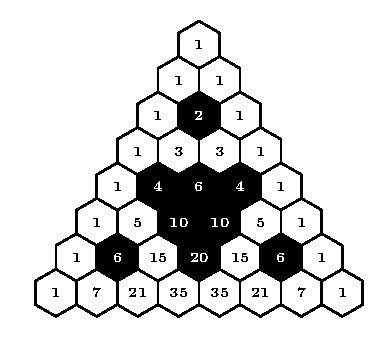
\includegraphics[scale=0.8]{Mod2,7.pdf}
    \end{figure}
    % Insert an image of pascal with seirpinski gasket
    

\end{frame}

\begin{frame}
    \begin{figure}
        \centering 
        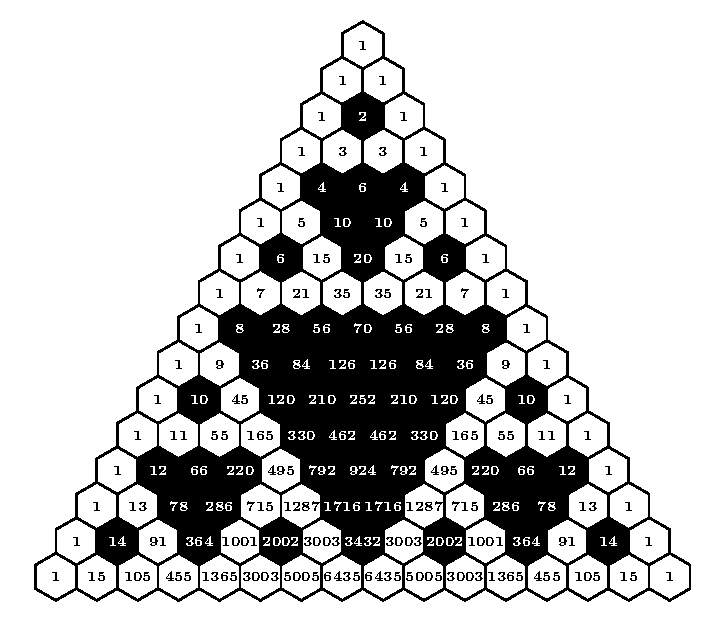
\includegraphics[scale=0.8]{PascalMod2.pdf}
    \end{figure}
\end{frame}
%\begin{comment}
    

\begin{frame}
    \frametitle{Pascal's Triangle}
    \begin{itemize}
        \item
        Can also be formulated through binomial coefficients
        \begin{align*}
            (1+x)^{0} &=\qquad 1 \\
            (1+x)^{1} &=\quad 1+1 x \\
            (1+x)^{2} &= 1+2 x+1 x^{2} \\ & \vdots \\(1+x)^{n} &=a_{0}+a_{1} x+\cdots+a_{n} x^{n} 
        \end{align*}
        where coefficients are given by
        \begin{equation*}
            a_{k}= \binom{n}{k} =\frac{n !}{(n-k) ! k !}, \quad 0 \leq k \leq n
        \end{equation*}
    \end{itemize}
\end{frame}

\begin{frame}
    \frametitle{Pascal's Triangle}
    \begin{itemize}
        \item
        Understanding the divisibility of binomial coefficients by computing them is a bad idea
        \begin{align*}
            50! = &3041409320171337804361260816606476884437\\
            &7641568960512000000000000   
        \end{align*}
        Even if we use the recursive formula 
        \begin{equation*}
            \binom{n+1}{k}= \binom{n}{k-1} + \binom{n}{k}
        \end{equation*}
        \begin{equation*}
            \binom{40}{20} = 137846528820 > 2^{32}
        \end{equation*}
        which is a big number\\
        Fortunately, we don't need to compute these large numbers
        \end{itemize}
    
\end{frame}

\begin{frame}
    \frametitle{Pascal's Triangle}
    \begin{itemize}
        \item
        Ex: Divisibility by 2 can be followed from addition rule 
        \begin{table}[H]
            \begin{tabular}{|l|l|l|}
                \hline
                $\binom{n}{k-1}$& $\binom{n}{k}$& $\binom{n+1}{k}$\\
                \hline
                even & even & even \\
                odd  & even & odd  \\
                even & odd  & odd  \\
                odd  & odd  & odd\\
                \hline
            \end{tabular}
        \end{table}
        \item
        Can we extend this idea of divisibility to other numbers ?
        \item
        What patterns do we get ? Global pattern? Why? ...IFS
    \end{itemize}
\end{frame}
\section{Cellular Automata}
%\begin{comment}

\begin{frame}
    \frametitle{Cellular Automata}
    \begin{itemize}
        \item
        Prefect feedback machines. They are mathematically finite state machines
        \item
        Each cell has one out of $p$ states. \textit{p-state} automata
        \item
        Can be 1D, 2D \dots
        \item
        To run cellular automata, we need 2 pieces of information 
        \begin{enumerate}
            \item Initial state of cells 
            \item Rules to describe new cell state from the states of a group of cells from the previous layer 
        \end{enumerate}
        \item The rules should not depend on the position of the group of cells within the layer.
        \begin{figure}
            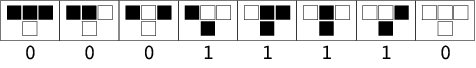
\includegraphics[scale = 0.5]{fig1.png} 
        \end{figure}
    \end{itemize}
\end{frame}

\begin{frame}
    \frametitle{Cellular Automata}
    \begin{itemize}
        \item More kinds of rules
        \begin{figure}[H]
            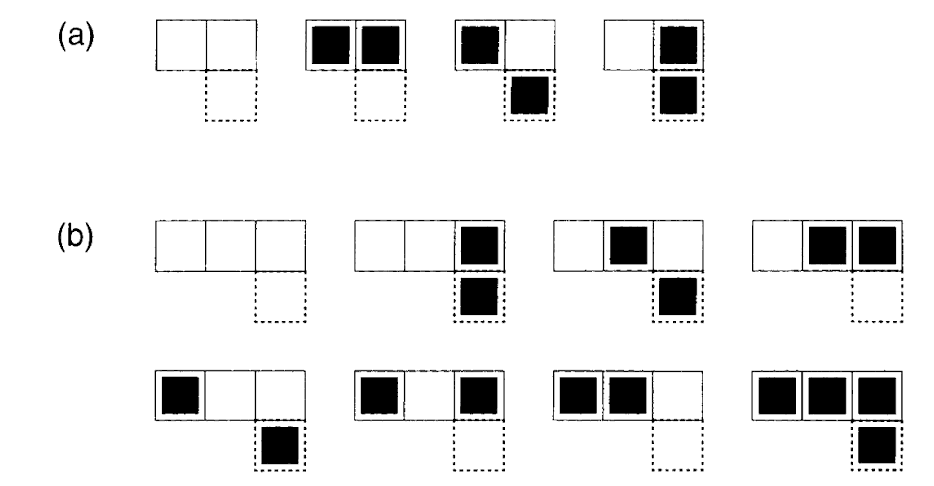
\includegraphics[scale = 0.37]{fig2}
            \caption{(a) is a four rule configuration and (b) is a 8 rule configuration}
        \end{figure}
    \end{itemize}
\end{frame}

\begin{frame}
    \frametitle{Cellular Automata}
    So lets run some 
    \begin{figure}
        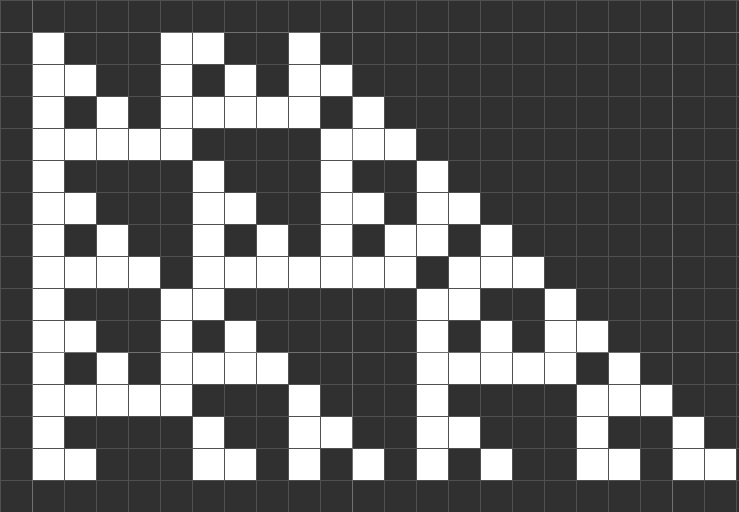
\includegraphics[scale=0.4]{fig3.png}
        \caption{13 Generations of Rule 60 Elementary CA}
    \end{figure}
\end{frame}
\subsection{Elementary CA}
\begin{frame}
    \frametitle{Elementary Cellular Automata}
    \begin{itemize}
        \item Simplest form of 1D Cellular Automata (CA)
        \item 2 State CA
        \item Next generation depends on itself,cell to the left and, cell to the right.
        \item Total number of rules are $2^{2^3} = 256$
        \item All the rules can be numbered in a nice way using binary
        \begin{figure}[H]
            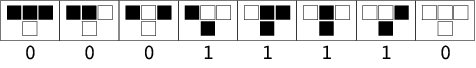
\includegraphics[scale=0.5]{fig1.png}
            \caption{Elementary rule 30 = $(00011110)_2$}
        \end{figure}
        \item Mathematica can do this for you very easily using CellularAutomaton[ ]
    \end{itemize}
\end{frame}

\begin{frame}
    \frametitle{Elementary Cellular Automata}
    \begin{figure}
        \centering
        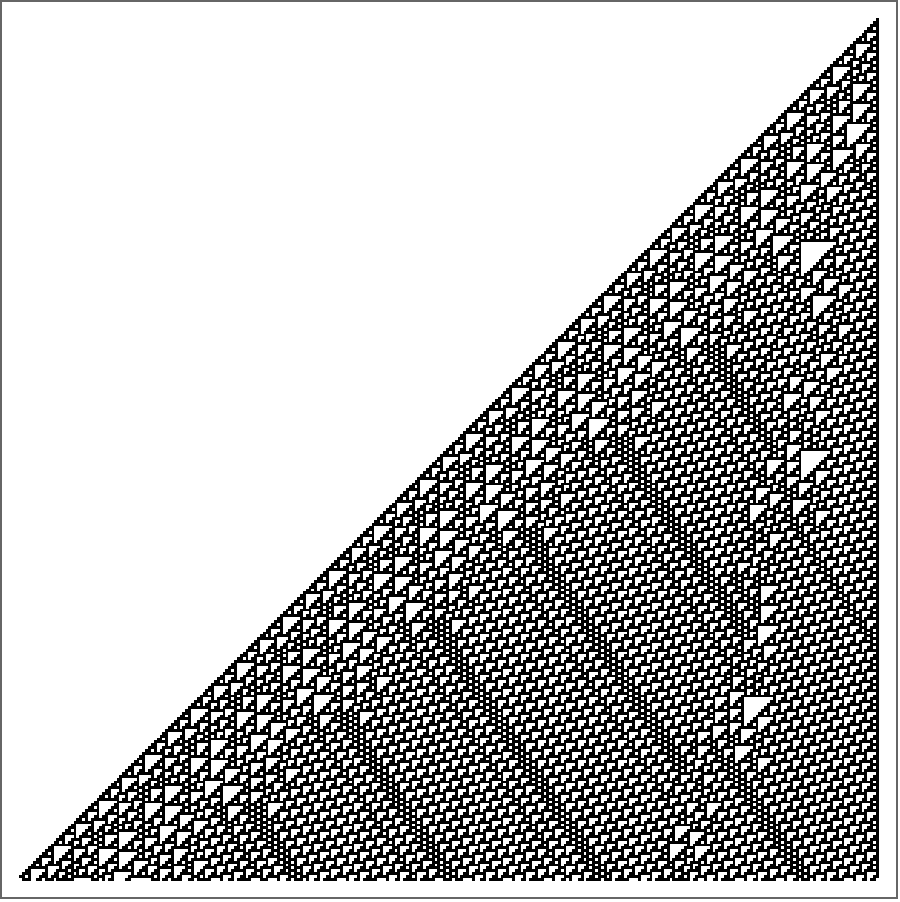
\includegraphics[scale=0.45]{fig4.pdf}
        \caption{Rule 110, this might be special}
    \end{figure}
\end{frame}

\begin{frame}
    \frametitle{Elementary Cellular Automata}
    \begin{figure}
        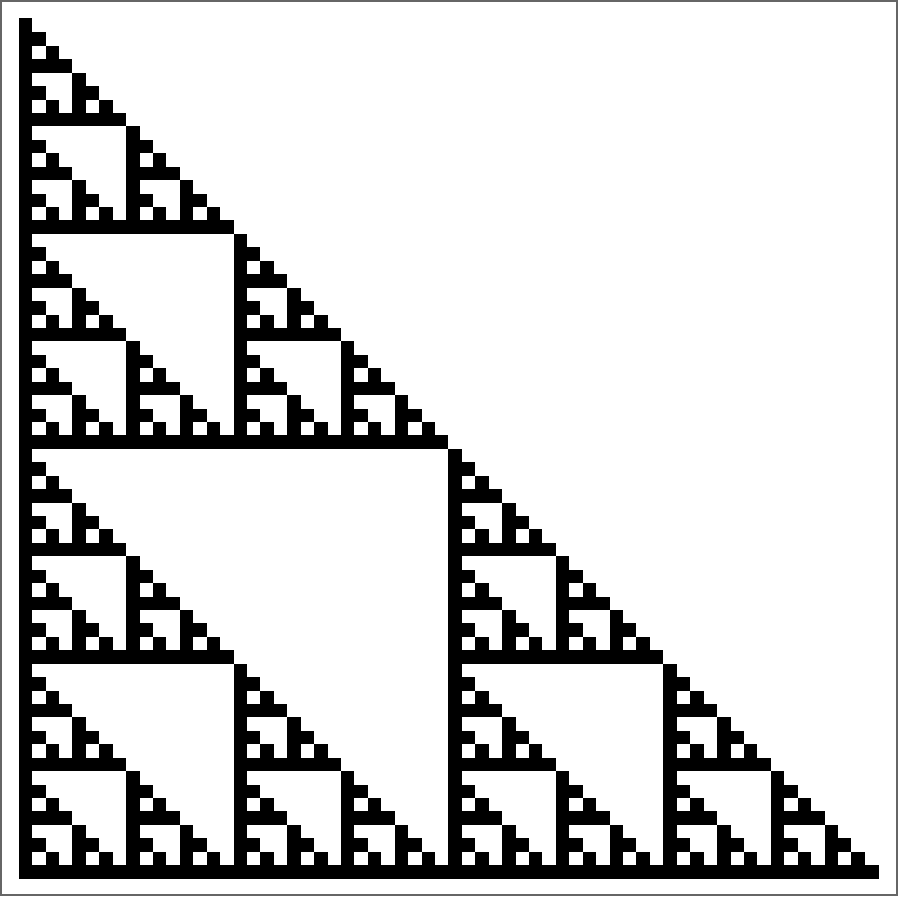
\includegraphics[scale=0.45]{seir.pdf}
        \caption{Rule 60. Sierpinski Triangle*}
    \end{figure}
\end{frame}

\begin{frame}
    \frametitle{Elementary Cellular Automata}
    \begin{figure}
        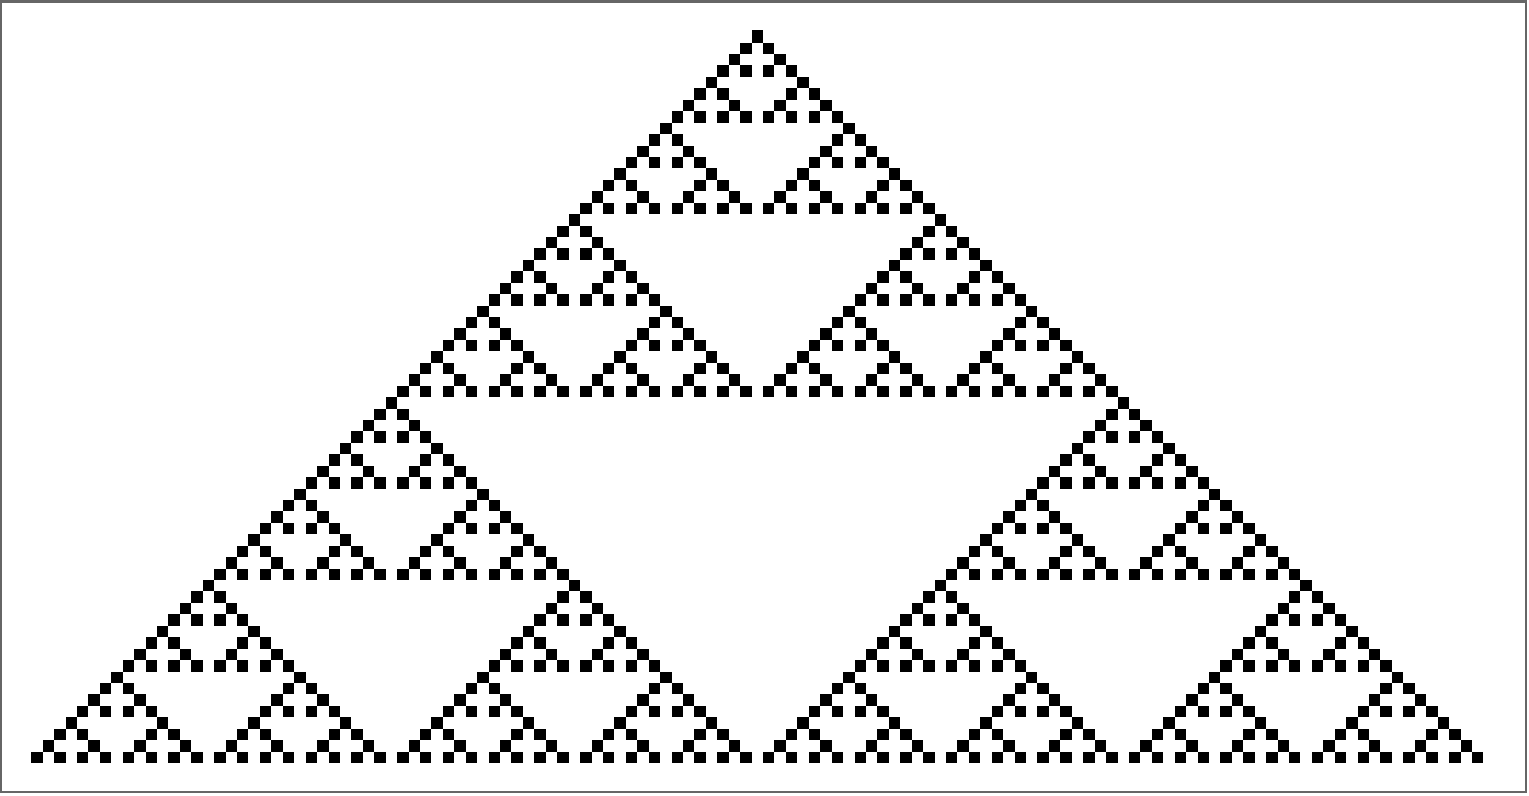
\includegraphics[scale=0.4]{sier2.pdf}
        \caption{Rule 90.}
    \end{figure}
\end{frame}

\begin{frame}
    \frametitle{Elementary Cellular Automata}
    \begin{figure}
        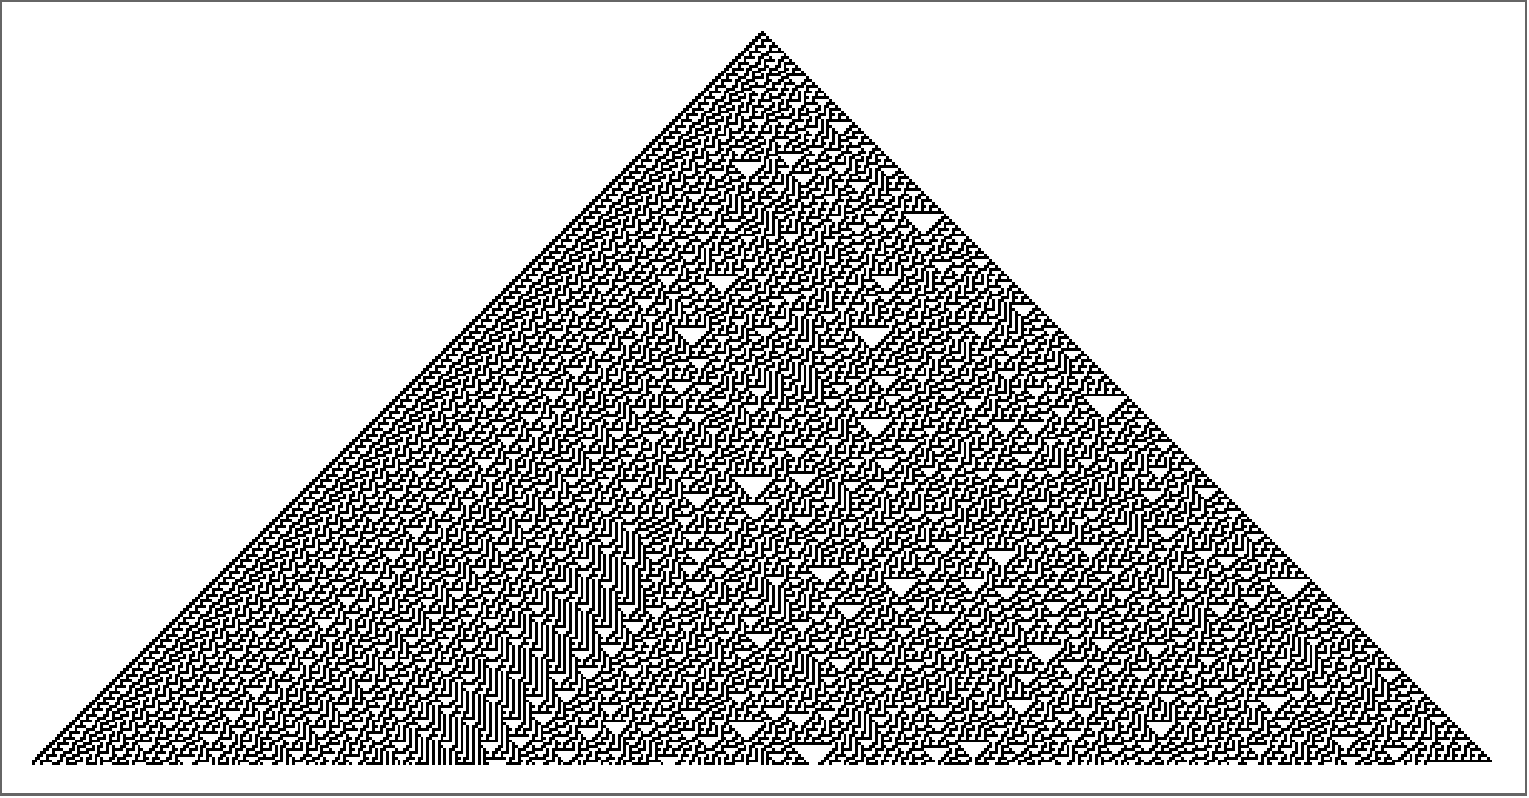
\includegraphics[scale=0.39]{rule30.pdf}
        \caption{Rule 30}
    \end{figure}
    Kinda chaotic ?
\end{frame}
\subsection{2D CA}
\begin{frame}
    \frametitle{2D CA: Game of life...}
    \begin{itemize}
        % Maybe I can ger rid of this one 
        \item Was very popular through the work of John Horton Conway in 1970's
        \item 2-state CA
        \item Rules:
        \begin{enumerate}
            \item Cell survives when exactly 2 or 3 of it's 8 neighbors are alive.
            \item If more than 3 neighbors are alive, the cell dies from overcrowdedness.
            \item If fewer than 2 neighbors are alive, the cell dies from oneliness.
            \item Dead cell comes back to life when surrounded by exactly 3 live neighbors.  
        \end{enumerate}
        \item Makes some interesting patters and life like behavior 
        \item Note:The position of the alive and dead cells w.r.t the center does not matter for this rule. Also known as Totalistic CA
    \end{itemize}
\end{frame}

\begin{frame}
    \centering
    Let's play the Game of Life......
\end{frame}

\begin{frame}
    \frametitle{Cellular Automata}
    \begin{itemize}
        \item Another variant of Game of Life: One out of eight rule
        \begin{enumerate}
            \item Cell becomes alive if exactly one neighbor is alive.
            \item Otherwise unchanged.
        \end{enumerate}
        \item Has some nice self-similarity
    \end{itemize}
\end{frame}

\begin{frame}
    \frametitle{Cellular Automata} 
    \begin{itemize}
        \item Game of life is just one out of the imaginable set of rules 
        \item For 2-state 2D automata and a neighborhood of eight cells, there are $2^{2^9} \approx 10^{154}$ different sets of rules!!
        \item Let's look at another rule: Majority Rule
        \begin{enumerate}
            \item If 5 or more of the neighborhood of 9 cells (including itself) are alive, this cell lives or stays alive 
            \item Otherwise dies or remains dead
        \end{enumerate}
        \item Here center cell adjusts to the majority 
        \item This kind of rule is called Outer Totalistic
        \item Has some resemblance with percolation
    \end{itemize}
\end{frame}

\begin{frame}
    \frametitle{Cellular Automata with Different neighbors}
    \begin{itemize}
        \item Let's consider only 4 neighbors.
        \begin{figure}
            \centering
            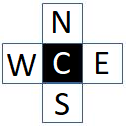
\includegraphics[scale=0.5]{VonNeigh.png}
        \end{figure}
        \item C = Center, N = North, E = East, S = South, W = West
        \item Can represent every neighbor in Binary $(\text{CSWNE})_2$. Ex:$(01100)_2$ means S, W cells are alive, rest are dead
        \item Total number of sets of rules are $2^{2^5} \approx 4 \cdot 10^9$
        \item Two interesting examples are shown 
    \end{itemize}
\end{frame}

\begin{frame}
    \frametitle{Cellular Automata}
    \begin{table}[H]
        \begin{tabular}{l|l|l|l|l|l|l|l}
        CSWNE & C & CSWNE & C & CSWNE & C & CSWNE & C \\
        \hline
        00000 & 0 & 01000 & 1 & 10000 & 1 & 11000 & 1 \\
        00001 & 0 & 01001 & 1 & 10001 & 1 & 11001 & 1 \\
        00010 & 0 & 01010 & 1 & 10010 & 1 & 11010 & 1 \\
        00011 & 0 & 01011 & 1 & 10011 & 1 & 11011 & 1 \\
        00100 & 1 & 01100 & 0 & 10100 & 1 & 11100 & 1 \\
        00101 & 1 & 01101 & 0 & 10101 & 1 & 11101 & 1 \\
        00110 & 1 & 01110 & 0 & 10110 & 1 & 11110 & 1 \\
        00111 & 1 & 01111 & 0 & 10111 & 1 & 11111 & 1
        \end{tabular}
    \end{table}
    \begin{itemize}
        \item This behaves like a 1D CA
    \end{itemize}
\end{frame}

% Maybe the last point is obvious and need not be stated 
\begin{frame}
    \frametitle{Cellular Automata}
    \begin{itemize}
        \item Many interesting rules can be given by a simple formula
        \item Parity Rule:
        \begin{equation*}
            C_{new} = C_{old} + N_{old} + E_{old} + S_{old} + W_{old} \mod 2
        \end{equation*}
        \item Again, this is a 2-state CA
    \end{itemize}
\end{frame}
\subsection{CA,Pascal's Triangle and Polynomials}
\begin{frame}
    \frametitle{CA, Pascal's Triangle and Polynomial}
    \begin{itemize}
        \item Let's look at the powers of $r(x) = 1 + x$:
        \begin{align*}
            (r(x))^{0} &=1 \\
            (r(x))^{1} &=1+x \\
            (r(x))^{2} &=1+2 x+x^{2} \\
            (r(x))^{3} &=1+3 x+3 x^{2}+x^{3} \\ & \vdots \\
            (r(x))^{n} &=a_{0}(n)+a_{1}(n) x+a_{2}(n) x^{2}+\cdots+a_{n}(n) x^{n} 
        \end{align*}
        \item By the addition rule of binomial coefficients
        \begin{equation*}
            a_k(n) = a_{k-1}(n-1) + a_k(n-1)
        \end{equation*}
        \item $a_k(n)$ gives the state of $\text{n}^{\text{th}}$ layer $\text{CA}^*$ 
    \end{itemize}
\end{frame}
% Need to bring changes to this slide 
% Maybe add a figure to give better explanation of last point
\begin{frame}
    \frametitle{CA, Pascal's Triangle and Polynomial}
    \begin{itemize}
        \item Looking at the divisibility properties of $a_k(n)$ with 2
        \begin{align*}
            a_k(n) \equiv 0 \pmod 2  \qquad or&& a_k(n) \equiv 1 \pmod 2
        \end{align*}
        \item With this, the addition rules in mod 2 arithmetic simplifies to
        \begin{table}
            \centering
            \begin{tabular}{|c|c|c|}
                \hline
                $\binom{n}{k-1}$& $ \ \binom{n}{k} \ $ & $\binom{n+1}{k}$\\
                \hline
                0 & 0 & 0 \\
                1  & 0 & 1  \\
                0 & 1  & 1  \\
                1  & 1  & 0\\
                \hline
            \end{tabular}
        \end{table}
        \item Exactly same rule set used to make Pascal Triangle
        \item Thus, that figure shows the coefficients of the power of $r(x) = 1+x \mod 2$ 
    \end{itemize}
\end{frame}

\begin{frame}
    \frametitle{Generalizations}
    \begin{itemize}
        \item There are 2 ways to generalize,
        \begin{enumerate}
            \item A different coefficient modulo integer 
            \item A different polynomial
        \end{enumerate}
        \item Ex: Let $r(x) = 1+2x$
        \begin{align*}
            (r(x))^0 &= 1 \\
            (r(x))^1 &= 1+2x \\
            (r(x))^2 &= 1 + 4x + 4x^2\\
            %(r(x))^3 &= 1 + 6x + 12x^2 + 8x^3 \\
            &\vdots \\
            (r(x))^n &= a_0(n) + a_1(n)x + \dots + a_n(n)x^n
        \end{align*}
        \item By pattern
        \begin{equation*}
            a_k(n) = a_{k}(n-1) + 2a_{k-1}(n-1)
        \end{equation*}
    \end{itemize}
\end{frame}

\begin{frame}
    \begin{itemize}
        \item By looking at the divisibility property with p = 3, we get 
        \begin{align*}
            (r(x))^0 &= 1 \\
            (r(x))^1 &= 1 \ 2 \\
            (r(x))^2 &= 1 \ 1 \ 1 \\
            (r(x))^3 &= 1 \ 0 \ 0 \ 2
        \end{align*}
        \item The cellular automaton would be $a_{n,k} = a_{n-1,k} + 2a_{n-1,k-1} \mod 3$
        \begin{figure}
            \centering
            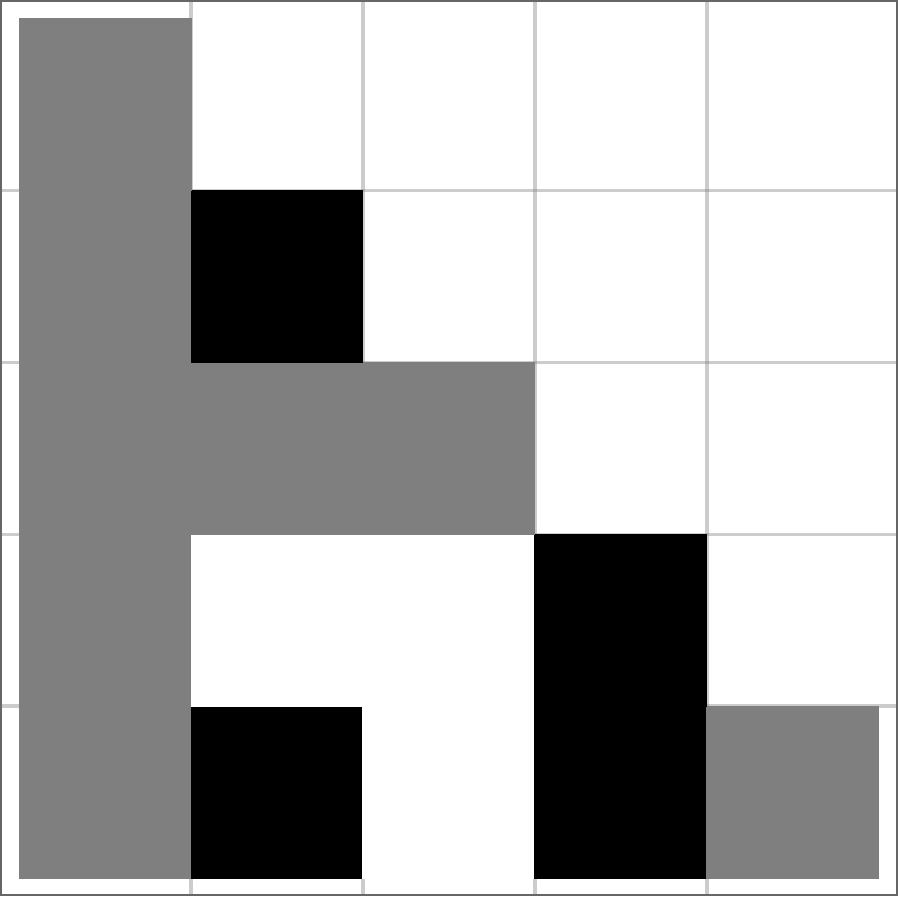
\includegraphics[scale=0.2]{Mod3Poly.pdf}
            \caption{CA for $r(x) = 1 + 2x \mod 2$}
        \end{figure}
    \end{itemize}
\end{frame}

\begin{frame}
    \frametitle{Linear Cellular Automata}
    \begin{itemize}
        \item We can start with any polynomial $r(x) = a_0 + a_1x+\dots+a_dx^d$
        \item The coefficients of $(r(x))^n$ modulo some positive integer $p$ is obtained by an addition formula involving $d$ coefficients from              $(r(x))^{n-1}$
        \item So, there is an associated Cellular Automata which generates coefficients modulo p of the powers of $(r(x))^n$
        \item A look-up table can be generated by an addition formula
        \item These are called \textit{Linear Cellular Automata}
        \item Again, the choice of p determines the number of states.
        This opens up a lot of interesting problems 
    \end{itemize}
\end{frame}

\begin{frame}
    \begin{itemize}
        \item Pattern Formation: Given a polynomial, what is the global pattern which evolves when the automaton has run for a long time?
        \item Colors: What is the relation between the global patterns which are obtained for different choices of p?
        \item Fractal Dimension: Fractal dimension of the global pattern ?
        \item Higher Dimension: What if we used polynomial of m variables ? (m-dimensional ?)
        \item Factorization: If a polynomial $r(x)$ can be factorized to two polynomials $s(x)$ and $t(x)$, how are the patters related ? Is that factorization unique ? \\
        In general, no, it depends on $p$\\
        Ex: $1+x$ is irreducible with respect to integers. But in arithmetic modulo $p$, with $p$ not prime, there are non trivial factorization
        \begin{equation*}
            1+x \equiv (1+3x)(1+4x) \pmod 6
        \end{equation*}
    \end{itemize}
\end{frame}

\section{Binomial Coefficients and Divisibility}
\begin{frame}
    \frametitle{Binomial Coefficients and Divisibility}
    \begin{itemize}
        \item Discuss the question of whether a binomial coefficient is divisible by $p$ or not. 
        \item Black and white coloring of the Pascal triangle depending on divisibility with p
        \item We will also see that in order to understand the patterns formed by mod $p$, we should look at the patters formed by the prime factors of $p$ 
        \item We will look at a direct, non-recursive computation of divisibility by p
        \item This was solved in an elegant manner by Ernest Eduard Kummer.
    \end{itemize}
\end{frame}

\begin{frame}
    \begin{figure}
        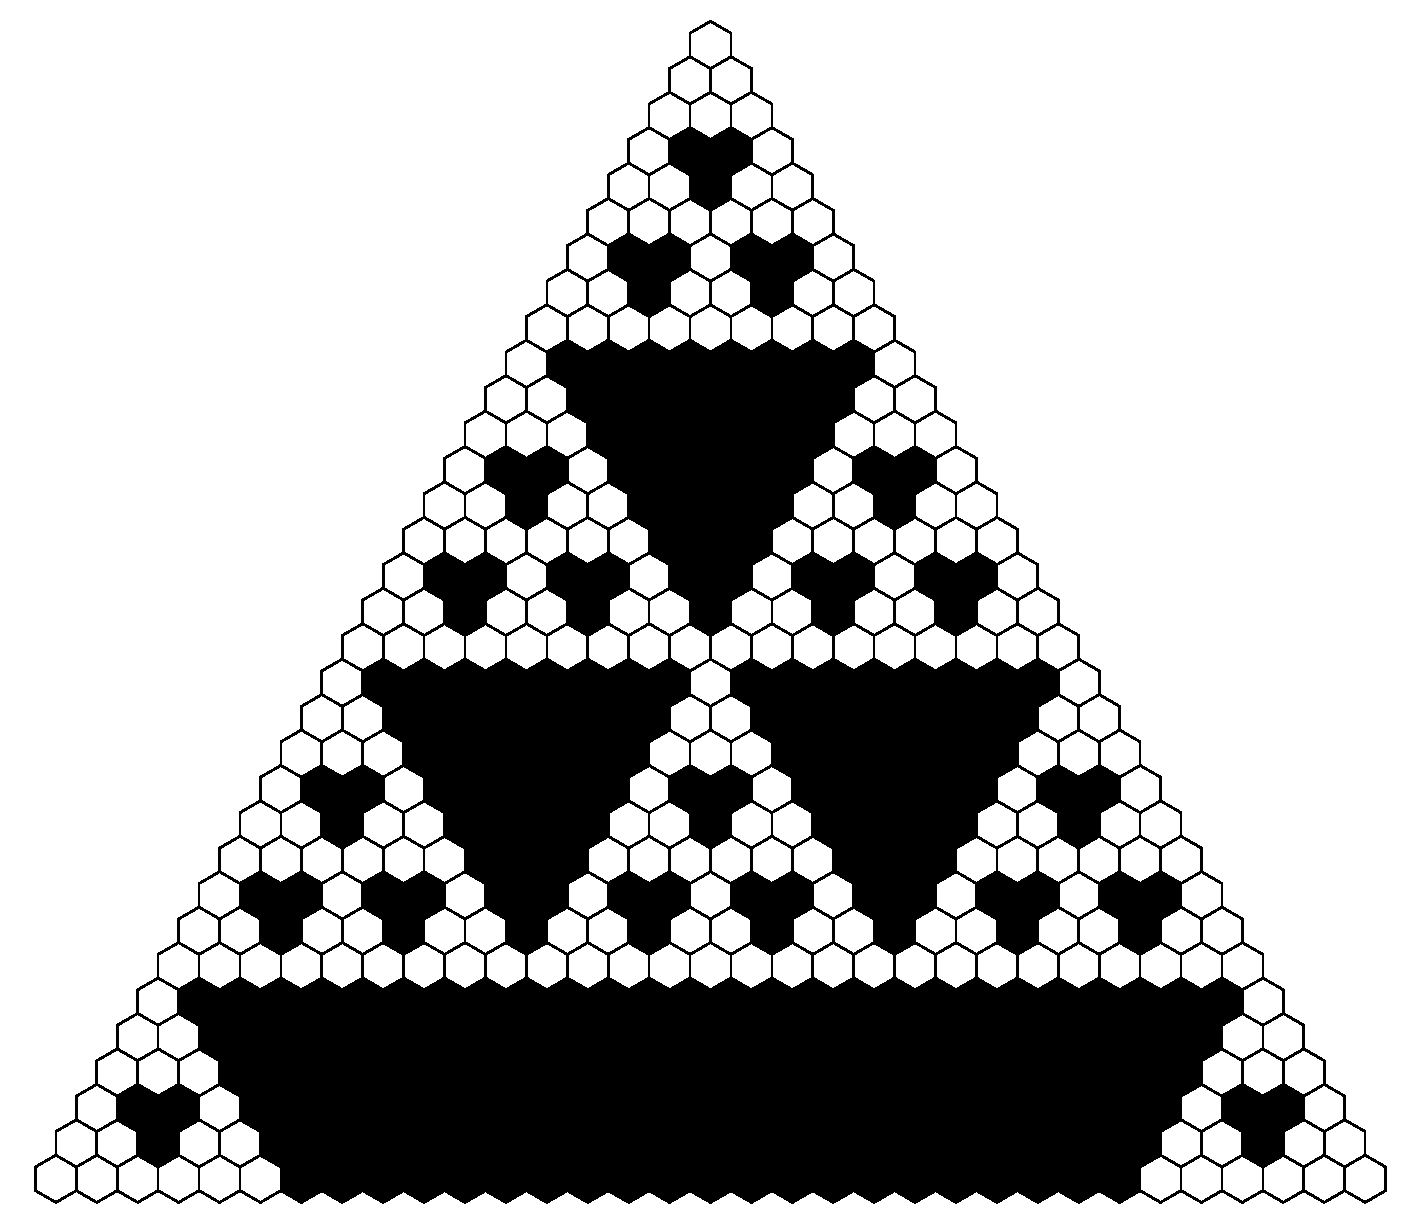
\includegraphics[scale=0.37]{PascalMod3.pdf}
        \caption{Pascal triangle Mod 3}
    \end{figure}
\end{frame}

\begin{frame}
    %\frametitle{Binomial Coefficients and Divisibility}
    \begin{itemize}
        \item We define a new coordinate system such that, at position $(n,k)$ the binomial coefficient is 
        \begin{equation*}
            \binom{n+k}{k} = \frac{(n+k)!}{n!k!}
        \end{equation*}
        \begin{figure}
            \centering
            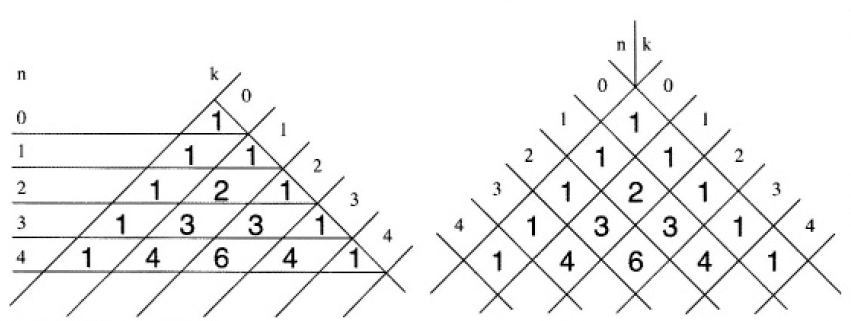
\includegraphics[scale=0.39]{newCoordinate.png}
            \caption{A new coordinate system}
        \end{figure}
    \end{itemize}
\end{frame}

\subsection{Divisibility Sets}
\begin{frame}
    \frametitle{Divisibility Sets}
    \begin{itemize}
        \item We formally define our problem
        \begin{equation*}
            P(r) = \left\{ (n,k) \left| \binom{n+k}{n} \text{ is not divisible by }r \right. \right\}
        \end{equation*}
        \item Observe that if $p$ and $q$ are two different prime numbers and a given integer $r$ is \textbf{not} divisible by $p \cdot q$, then it is \textbf{not} divisible by either $p$ or $q$
        \begin{equation*}
            P(pq) = P(p) \cup P(q) \text{, if $p \neq q$, $p,q$ prime}
        \end{equation*}
        \item It is the negation of the statement, if $p$ and $q$ divides $r$, then $r$ is divisible by both $p$ and $q$.
        \item Ex: $P(6) = P(3) \cup P(2)$. This generalization can be extended to any integer
    \end{itemize}
\end{frame}

\begin{frame}
    \begin{figure}
        \centering
        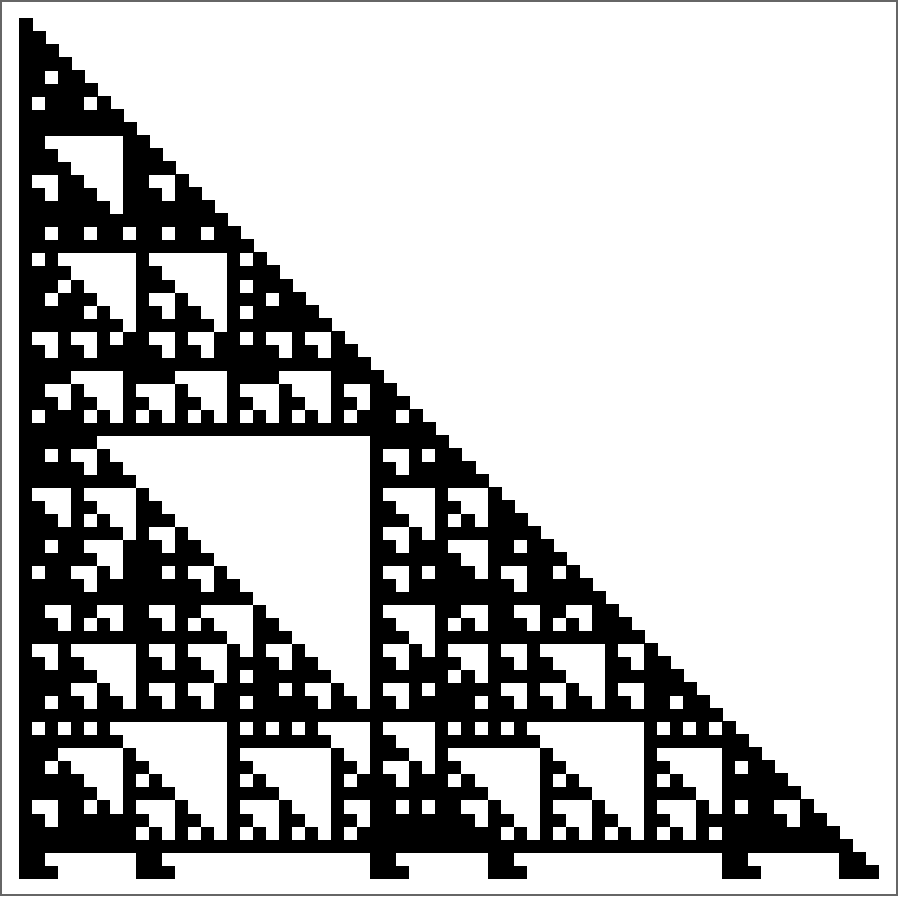
\includegraphics[width=0.475\textwidth]{Mod6.pdf}
        \hfill
        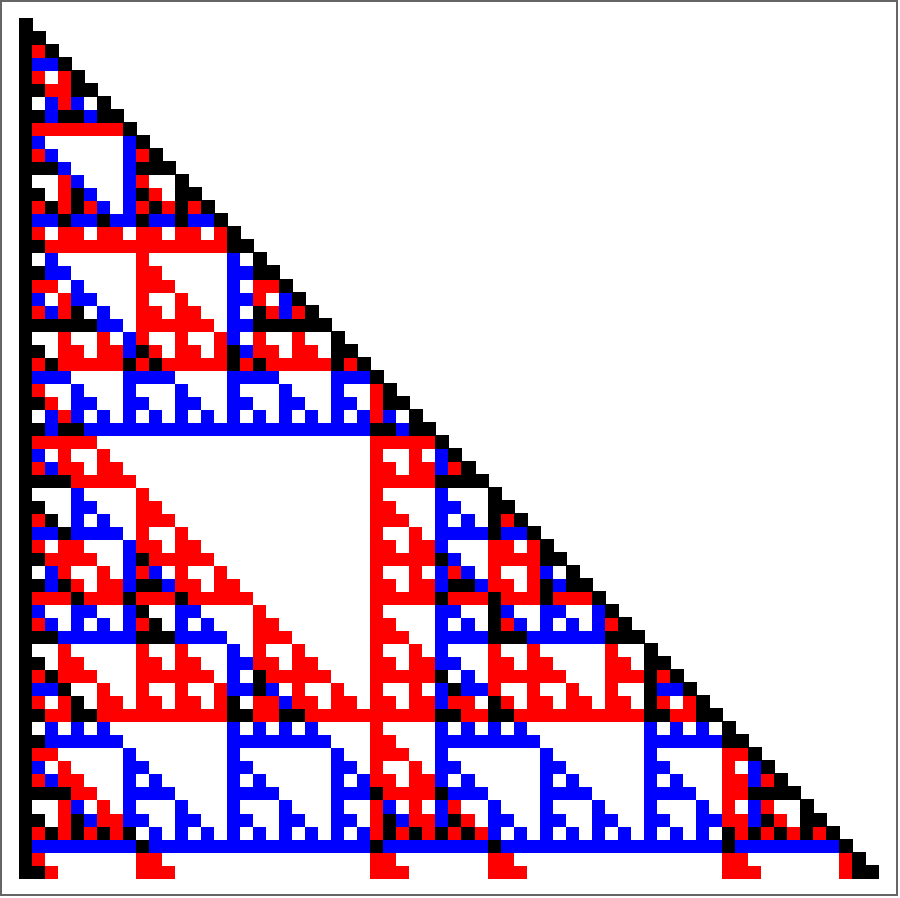
\includegraphics[width=0.475\textwidth]{mod2,3.pdf}
        \caption{Right shows mod 6 pattern and left shows the union of mod 2 (Red) and mod 3 (Blue)}
    \end{figure}
\end{frame}

\begin{frame}
    \begin{itemize}
        \item For an integer $r = p_1^{n_1}\dots p_s^{n_s}$ where $p_1,\dots,p_s$ are primes
        \begin{equation*}
            P(r) = P(p_1^{n_1}) \cup ... \cup P(p_s^{n_s})
        \end{equation*}
        \item So to understand the pattern formed by $P(r)$, we just need to understand the pattern of $P(p^n)$
    \end{itemize}
\end{frame}

\subsection{Kummer's Result}
\begin{frame}
    \frametitle{Kummer's Result and p-adic numbers}
    \begin{itemize}
        \item To understand Kummer's result, we need to consider numbers with base $p$, where $p$ is prime 
        \item Like the decimal system, p-adic expansion of an integer is given by
        \begin{equation*}
            n = a_0 + a_1p +\dots + a_m p^m
        \end{equation*}
        where $a_i \in \{0,1,\dots,p-1\}$
        \item The p-adic representation would be 
        \begin{equation*}
            n = (a_m a_{m-1} \dots a_0)_p
        \end{equation*} 
        \item Ex: $15_{10} = (1111)_2 = (120)_3 = (30)_5 = (21)_7 = (14)_{11}$ 
    \end{itemize}
    
\end{frame}

\begin{frame}
    \begin{itemize}
        \item We define carry function $c_p$
        \begin{equation*}
            c_p(n,k) = \text{number of carries in the p-adic addition of n and k}
        \end{equation*}
        \item Ex: For $n = 15$ and $k=8$
        \begin{equation*}
            k=(08)_{10}=(1000)_{2}=(022)_{3}=(13)_{5}=(11)_{7}=(08)_{11}
        \end{equation*}
        \item If we take the binary addition
        \begin{tabular}{cccccc}
            & $0$ & $1$ & $1$ & $1$ & $1$ \\
            + & $0_1$ & $1$ & $0$ & $0$ & $0$ \\
            \hline
            & $1$ & $0$ & $1$ & $1$ & $1$ 
        \end{tabular}
        \begin{equation*}
            c_2(15,8) = 1
        \end{equation*}
        \item Similarly, we can do the same for $p=3,5,7\dots$
    \end{itemize}
\end{frame}

\begin{frame}
    \frametitle{Kummer's result}
    \begin{itemize}
        \item Let $\tau = c_p(n,k),$ then $\binom{n+k}{k}$ is divisible by $p^\tau$ but not $p^{\tau + 1}$
        \item So, prime factorization of $\binom{n+k}{k}$ contains exactly $c_p(n,k)$ factors of $p$
        \item This result is pretty amazing, since it gives a direct method to check if a binomial coefficient is divisible by $p$ or not.
        \item For $n=15$ and $k=8$
        \begin{equation*}
            \binom{15+8}{8} = \binom{23}{8} = 2 \cdot 3 \cdot 11 \cdot 17 \cdot 19 \cdot 23
        \end{equation*} 
        \item So the Kummer's result implies 
        \begin{equation*}
            c_{p}(17,8)=\left\{\begin{array}{l}{1, \text { for } p=2,3,11,17,19} \\  {0, \text { otherwise }}\end{array}\right.
        \end{equation*}
    \end{itemize}
\end{frame}

\begin{frame}
    \begin{itemize}
        \item Applying Kummer's result to Divisibility Set gives 
        \begin{equation*}
            P(p) = \{(n,k) | \ c_p(n,k) = 0\}
        \end{equation*}
        \item That is, the number of carries $c_p(n,k)$ is only $0$ if and only if 
        \begin{equation*}
            a_i + b_i < p, \quad i = 0,\dots,m
        \end{equation*}
        where $a_i$ and $b_i$ are the p-adic digits of n and k. 
        \item This is called the \textit{mod-p} condition.
        \item For prime powers, 
        \begin{equation*}
            P(p^\tau) = \{(n,k)| \ c_p(n,k) < \tau \}
        \end{equation*}
    \end{itemize}
\end{frame}
\section{Iterated Function System}
\begin{frame}
    \frametitle{Iterated Function System}
    \begin{itemize}
        \item It is a method of constructing fractals using a set of contraction mappings. 
        \item A contraction mapping is an affine linear transformation 
        \begin{equation*}
            f(x, y)=\left[ \begin{array}{ll}{a} & {b} \\ {c} & {d}\end{array}\right] \left[ \begin{array}{l}{x} \\ {y}\end{array}\right]+\left[ \begin{array}{l}{e} \\ {f}\end{array}\right]
        \end{equation*}
        \item Union of these contraction mapping gives the Hutchinson equation of the fractal
        \item If you put a probability factor to these contraction mappings, you get some pretty images. 
    \end{itemize}
\end{frame}

% Some pretty pictures and some details about them 

\begin{frame}
    \begin{itemize}
    \item The Hutchinson operator for Sierpinski Triangle is:
    \begin{equation*}
        S = w_{00}(S) \cup w_{01}(S) \cup w_{10}(S)
    \end{equation*}
    where $w_{ij}$ are contraction mappings of a unit square
    \begin{align*}
        w_{00} &= (x/2,y/2)\\
        w_{01} &= (x/2, y/2+1/2) \\
        w_{10} &= (x/2 + 1/2, y/2) \\
        w_{11} &= (x/2 + 1/2 + y/2 + 1/2)
    \end{align*}
    \item So how do we know for sure that our Pascal Sierpinski triangle is the same as the Hutchinson operator Sierpinski Triangle?
    \item Let's construct Mod 2 Pascal triangle in a unit square 
    \end{itemize}
\end{frame}

\begin{frame}
    \begin{itemize}
        \item Let $Q$ be the unit square 
        \begin{equation*}
            Q = \{(x,y) | \ (x,y) \in [0,1] \times [0,1]\}
        \end{equation*}
        \item Expand $x$ and $y$ in base 2
        \begin{align*}
            x &= \sum_{i=1}^\infty a_i 2^{-i}, \ a_i \in \{0,1\} \\
            y &= \sum_{i=1}^\infty b_i 2^{-i}, \ b_i \in \{0,1\}
        \end{align*}
        \item From Kummer's result, we know that the coordinates of the points divisible by 2 are those which have no carries in the binary addition of the coordinates
        \begin{equation*}
            S = \{(x,y) \in Q| \ a_i + b_i \leq 1 \ \forall i\}
        \end{equation*} 
    \end{itemize}
\end{frame}

\begin{frame}
    \frametitle{Proof by picture}
\end{frame}

\begin{frame}
    \frametitle{Proof by symbols}
    \begin{itemize}
        \item To show both are the same, we need to show
        \begin{equation*}
            w_{00}(S) \cup w_{01}(S) \cup w_{10}(S) \subset S 
        \end{equation*}
        and, 
        \begin{equation*}
            w_{00}(S) \cup w_{01}(S) \cup w_{10}(S) \supset S
        \end{equation*}
        \item Take any point $(x,y) \in S$ 
        \begin{equation*}
            (x,y) = (0,a_1a_2a_3\dots,0.b_1 b_2 \dots)
        \end{equation*}
        where $a_i + b_i \leq 1$
        \item Applying the 3 transformations gives 
        \begin{align*}
            w_{00}(0,a_1a_2\dots,0.b_1 b_2 \dots) &= (0.0a_1a_2\dots,0.0b_1 b_2 \dots) \\
            w_{01}(0,a_1a_2\dots,0.b_1 b_2 \dots) &= (0.0a_1a_2\dots,0.1b_1 b_2 \dots) \\
            w_{10}(0,a_1a_2\dots,0.b_1 b_2 \dots) &= (0.1a_1a_2\dots,0.0b_1 b_2 \dots)
        \end{align*}
    \end{itemize}
\end{frame}
%\end{comment}

\begin{frame}
    \begin{itemize}
        \item Clearly, all these points are also in $S$.
        \item To show the second relation, we take any point $(x,y) \in S$, and we have to provide another point $(x',y') \in S$ such that $(x,y)$ is one of the images of $w_{00}(x',y'),w_{10}(x',y'),$ or $w_{01}(x',y')$. We choose 
        \begin{equation*}
            (x',y') = (0.a_2\dots,b_2\dots)
        \end{equation*}
        \item We obtain 
        \begin{equation*}
            (x, y)=\left\{\begin{array}{l}{w_{00}\left(x^{\prime}, y^{\prime}\right) \text { if } a_{1}=0 \text { and } b_{1}=0 \text { or }} \\ {w_{01}\left(x^{\prime}, y^{\prime}\right) \text { if } a_{1}=0 \text { and } b_{1}=1 \text { or }} \\ {w_{10}\left(x^{\prime}, y^{\prime}\right) \text { if } a_{1}=1 \text { and } b_{1}=0}\end{array}\right.
        \end{equation*}
        \item This completes our proof.
    \end{itemize}
\end{frame}

\begin{frame}
    \frametitle{Concequences}
    \begin{itemize}
        \item The binary representation allows us to see Hutchinson operator in action applied to a point inside square
        \item If $(x,y)$ is an arbitrary point in $Q$, the applying the map $w_{00},w_{01},w_{10}$ again and again yields points with leading binary decimal points satisfying $a_i + b_i \leq 1$
        \item In symbols,
        \begin{equation*}
            A_0 = Q
        \end{equation*} 
        Then running the IFS gives 
        \begin{equation*}
            A_n = w_{00}(A_{n-1}) \cup w_{01}(A_{n-1}) \cup w_{00}(A_{n-1})
        \end{equation*}
        where the leading $n$ binary digits satisfy $a_i + b_i \leq 1$
        \item Finally, the sequence will lead to Sierpinski triangle
        \begin{equation*}
            A_\infty = S
        \end{equation*}
    \end{itemize}
\end{frame}

\begin{frame}
    \frametitle{IFS for other primes}
    \begin{itemize}
        \item Now, we can finally look into the global pattern formation of divisibility of binomial coefficients with primes, i.e the global patterns formed by 
        \begin{equation*}
            P(r) = \left\{ (n,k) \left| \binom{n+k}{n} \text{is not divisible by }r \right. \right\}
        \end{equation*}
        \item We construct an IFS: Divide the unit square $Q$ in $p^2$ congruent square $Q_{a,b}$ with $a,b \in \{0,\dots,p-1\}$. We introduce the contraction mappings 
        \begin{equation*}
            w_{a,b}(x,y) = \left(\frac{x+a}{p}, \frac{y+b}{p}\right)
        \end{equation*} 
        where 
        \begin{equation*}
            w_{a,b}(Q) = Q_{a,b}
        \end{equation*}
    \end{itemize}
        
\end{frame}

\begin{frame}
    \begin{itemize}
        \item Then we set the restriction to define the set of transformation
        \begin{equation*}
            a+b \leq p-1
        \end{equation*}
        \item This restriction follows from Kummer's result,i.e $\binom{n+k}{n}$ is indivisible by $p$ when there is no carries in the p-adic addition of $n,k$
        \item The Hutchinson operator for these contractions,
        \begin{equation*}
            W_p(A) = \bigcup_{a+b < p} w_{a,b}(A)
        \end{equation*} 
    \end{itemize}
\end{frame}
\begin{comment}
\begin{frame}
    \begin{figure}
        \centering
        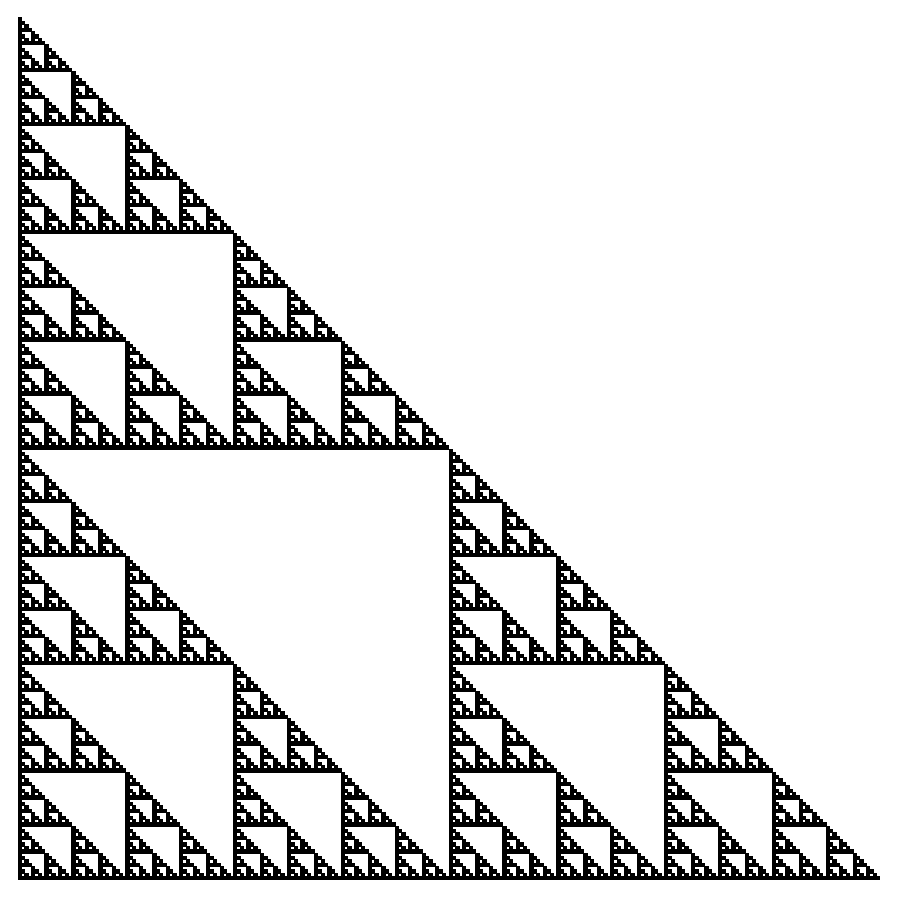
\includegraphics[scale=0.5]{GlobalMod2.pdf}
        \caption{Limit of Mod 2 IFS}
    \end{figure}
\end{frame}

\begin{frame}
    \begin{figure}
        \centering
        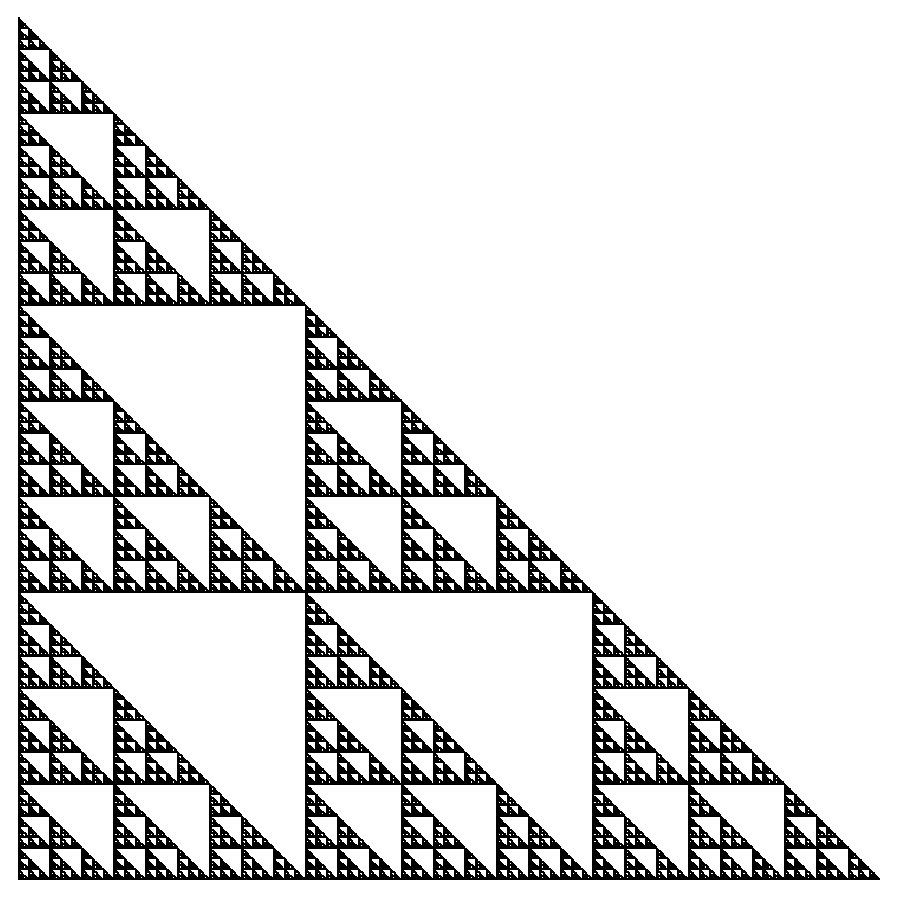
\includegraphics[scale=0.5]{GlobalMod3.pdf}
        \caption{Limit of Mod 3 IFS}
    \end{figure}
\end{frame}

\begin{frame}
    \begin{figure}
        \centering
        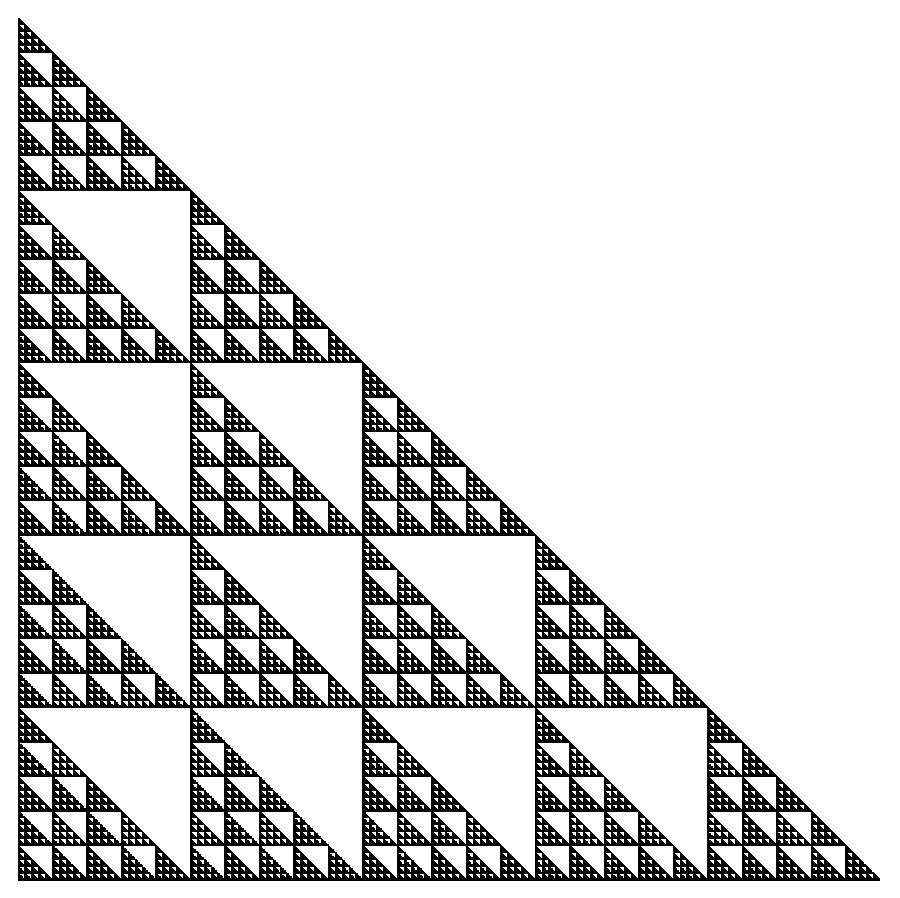
\includegraphics[scale=0.5]{GlobalMod5}
        \caption{Limit of Mod 5 IFS}
    \end{figure}
\end{frame}

\begin{frame}
    \begin{figure}
        \centering
        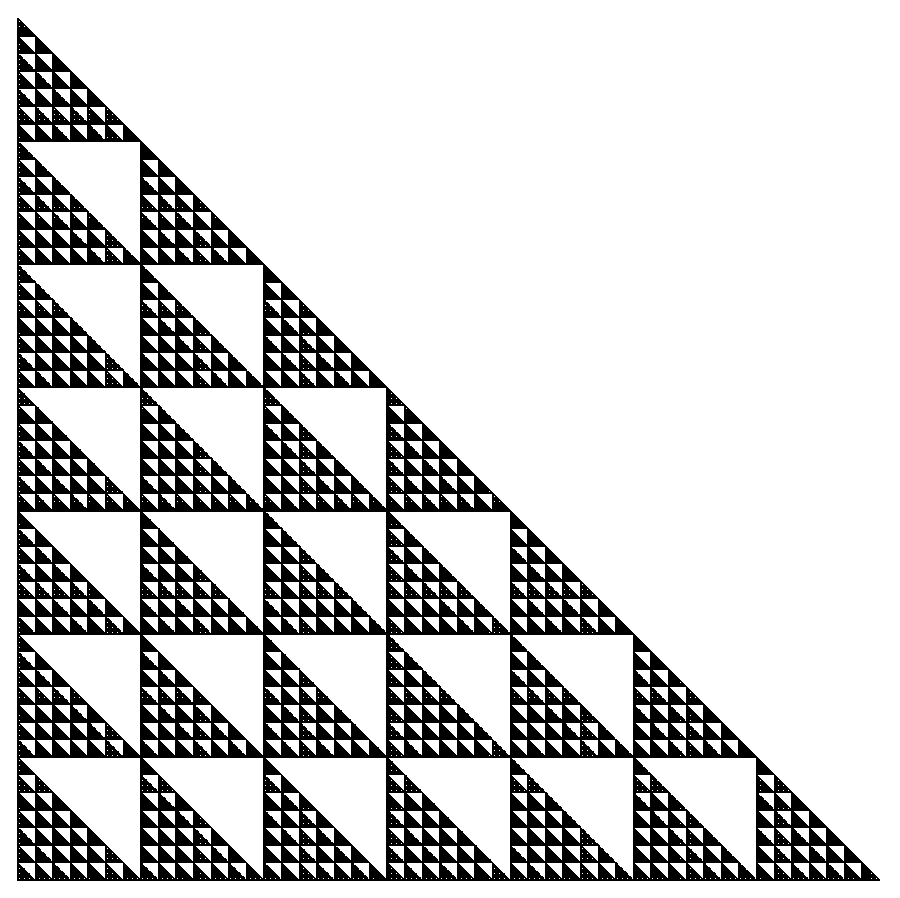
\includegraphics[scale=0.5]{GlobalMod7}
        \caption{Limit of Mod 7 IFS}
    \end{figure}
\end{frame}
\end{comment}
\section*{}
\begin{frame}
    \frametitle{Conlcusion}
    \begin{itemize}
        \item We approached the problem of coloring (or divisibility) of pascal's triangle in 3 different ways 
        \begin{enumerate}
            \item First, we looked at the macroscopic nature of divisibility, i.e how the neighbors affected the divisibility of a cell. We then explored the realm of cellular automata and how it extends this idea to general polynomials. We also peaked into some open ended problems
            \item Second, we looked at the microscopic nature of divisibility,i.e how the divisibility of a cell depends on its coordinate (Kummer's Result). We looked how p-adic numbers gave insight about binomial divisibility with primes. We also extended this idea of divisibility to all integers.
            \item Finally, we looked at the global pattern using Iterated function system. We showed that the limit of Pascal Mod 2 pattern was indeed the Sierpinski triangle. We also explored the global patterns of other primes and their IFS. 
        \end{enumerate}
    \end{itemize}
\end{frame}

\begin{frame}
    \begin{itemize}
        \item Each method gave a different perspective of the same problem.
        \item This entire chapter is trying to solve the jig-saw puzzle that relates fractals, Pascal's triangle, and Cellular Automata. 
        \item Understanding that these 3 very different things are all tied up by one common thread is, honestly, amazing. 
    \end{itemize}
\end{frame}

\end{document}